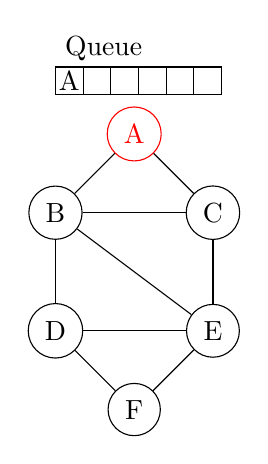
\begin{tikzpicture}
	\node [draw,circle,red] (node A) at (1,3.5) {A};
	\node [draw,circle] (node B) at (0,2.5) {B};
	\node [draw,circle] (node C) at (2,2.5) {C};
	\node [draw,circle] (node D) at (0,1) {D};
	\node [draw,circle] (node E) at (2,1) {E};
	\node [draw,circle] (node F) at (1,0) {F};
	
	\draw (node A) -- (node B);
	\draw (node A) -- (node C);
	\draw (node B) -- (node D);
	\draw (node B) -- (node E);
	\draw (node C) -- (node E);
	\draw (node D) -- (node F);
	\draw (node E) -- (node F);
	\draw (node B) -- (node C);
	\draw (node D) -- (node E);

	% The array under the graph
	%\foreach \x in{0,...,5}{\draw (\x*1em,-1) rectangle (\x*1em+1em,-1+1em);}
	\draw (0,4) rectangle (1em,4.35) node[pos=.5] {A};
	\draw (1em,4) rectangle (2em,4.35);
	\draw (2em,4) rectangle (3em,4.35);
	\draw (3em,4) rectangle (4em,4.35);
	\draw (4em,4) rectangle (5em,4.35);
	\draw (5em,4) rectangle (6em,4.35);

	\node [anchor=south west] at (0,4.3) {Queue};
\end{tikzpicture}
\hfill
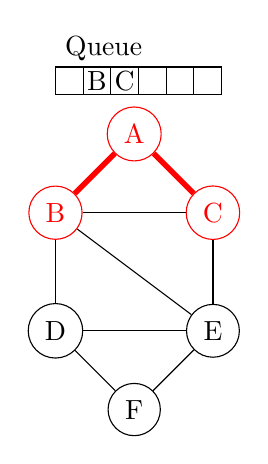
\begin{tikzpicture}
	\node [draw,circle,red] (node A) at (1,3.5) {A};
	\node [draw,circle,red] (node B) at (0,2.5) {B};
	\node [draw,circle,red] (node C) at (2,2.5) {C};
	\node [draw,circle] (node D) at (0,1) {D};
	\node [draw,circle] (node E) at (2,1) {E};
	\node [draw,circle] (node F) at (1,0) {F};
	
	\draw [red,line width=2pt] (node A) -- (node B);
	\draw [red,line width=2pt] (node A) -- (node C);
	\draw (node B) -- (node D);
	\draw (node B) -- (node E);
	\draw (node C) -- (node E);
	\draw (node D) -- (node F);
	\draw (node E) -- (node F);
	\draw (node B) -- (node C);
	\draw (node D) -- (node E);

	% The array under the graph
	%\foreach \x in{0,...,5}{\draw (\x*1em,-1) rectangle (\x*1em+1em,-1+1em);}
	\draw (0,4) rectangle (1em,4.35) node[pos=.5] {};
	\draw (1em,4) rectangle (2em,4.35) node[pos=.5] {B};
	\draw (2em,4) rectangle (3em,4.35) node[pos=.5] {C};
	\draw (3em,4) rectangle (4em,4.35) node[pos=.5] {};
	\draw (4em,4) rectangle (5em,4.35) node[pos=.5] {};
	\draw (5em,4) rectangle (6em,4.35) node[pos=.5] {};

	\node [anchor=south west] at (0,4.3) {Queue};
\end{tikzpicture}
\hfill
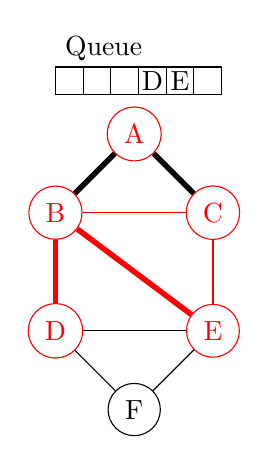
\begin{tikzpicture}
	\node [draw,circle,red] (node A) at (1,3.5) {A};
	\node [draw,circle,red] (node B) at (0,2.5) {B};
	\node [draw,circle,red] (node C) at (2,2.5) {C};
	\node [draw,circle,red] (node D) at (0,1) {D};
	\node [draw,circle,red] (node E) at (2,1) {E};
	\node [draw,circle] (node F) at (1,0) {F};
	
	\draw [line width=2pt] (node A) -- (node B);
	\draw [line width=2pt] (node A) -- (node C);
	\draw [red,line width=2pt] (node B) -- (node D);
	\draw [red,line width=2pt] (node B) -- (node E);
	\draw [red] (node C) -- (node E);
	\draw (node D) -- (node F);
	\draw (node E) -- (node F);
	\draw [red] (node B) -- (node C);
	\draw (node D) -- (node E);

	% The array under the graph
	%\foreach \x in{0,...,5}{\draw (\x*1em,-1) rectangle (\x*1em+1em,-1+1em);}
	\draw (0,4) rectangle (1em,4.35) node[pos=.5] {};
	\draw (1em,4) rectangle (2em,4.35) node[pos=.5] {};
	\draw (2em,4) rectangle (3em,4.35) node[pos=.5] {};
	\draw (3em,4) rectangle (4em,4.35) node[pos=.5] {D};
	\draw (4em,4) rectangle (5em,4.35) node[pos=.5] {E};
	\draw (5em,4) rectangle (6em,4.35) node[pos=.5] {};

	\node [anchor=south west] at (0,4.3) {Queue};
\end{tikzpicture}
\hfill
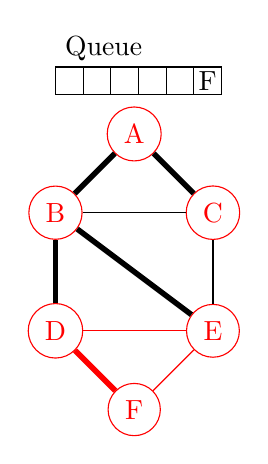
\begin{tikzpicture}
	\node [draw,circle,red] (node A) at (1,3.5) {A};
	\node [draw,circle,red] (node B) at (0,2.5) {B};
	\node [draw,circle,red] (node C) at (2,2.5) {C};
	\node [draw,circle,red] (node D) at (0,1) {D};
	\node [draw,circle,red] (node E) at (2,1) {E};
	\node [draw,circle,red] (node F) at (1,0) {F};
	
	\draw [line width=2pt] (node A) -- (node B);
	\draw [line width=2pt] (node A) -- (node C);
	\draw [line width=2pt]  (node B) -- (node D);
	\draw [line width=2pt] (node B) -- (node E);
	\draw (node C) -- (node E);
	\draw [red,line width=2pt] (node D) -- (node F);
	\draw [red] (node E) -- (node F);
	\draw (node B) -- (node C);
	\draw [red] (node D) -- (node E);

	% The array under the graph
	%\foreach \x in{0,...,5}{\draw (\x*1em,-1) rectangle (\x*1em+1em,-1+1em);}
	\draw (0,4) rectangle (1em,4.35) node[pos=.5] {};
	\draw (1em,4) rectangle (2em,4.35) node[pos=.5] {};
	\draw (2em,4) rectangle (3em,4.35) node[pos=.5] {};
	\draw (3em,4) rectangle (4em,4.35) node[pos=.5] {};
	\draw (4em,4) rectangle (5em,4.35) node[pos=.5] {};
	\draw (5em,4) rectangle (6em,4.35) node[pos=.5] {F};

	\node [anchor=south west] at (0,4.3) {Queue};
\end{tikzpicture}
\hfill
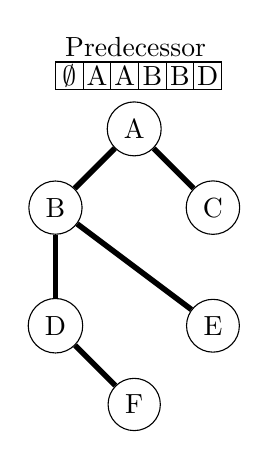
\begin{tikzpicture}
	\node [draw,circle] (node A) at (1,3.5) {A};
	\node [draw,circle] (node B) at (0,2.5) {B};
	\node [draw,circle] (node C) at (2,2.5) {C};
	\node [draw,circle] (node D) at (0,1) {D};
	\node [draw,circle] (node E) at (2,1) {E};
	\node [draw,circle] (node F) at (1,0) {F};
	
	\draw [line width=2pt] (node A) -- (node B);
	\draw [line width=2pt] (node A) -- (node C);
	\draw [line width=2pt] (node B) -- (node D);
	\draw [line width=2pt] (node B) -- (node E);
	\draw [line width=2pt] (node D) -- (node F);
	
	% The array under the graph
	%\foreach \x in{0,...,5}{\draw (\x*1em,-1) rectangle (\x*1em+1em,-1+1em);}
	\draw (0,4) rectangle (1em,4.35) node[pos=.5] {$\emptyset$};
	\draw (1em,4) rectangle (2em,4.35) node[pos=.5] {A}; % B
	\draw (2em,4) rectangle (3em,4.35) node[pos=.5] {A}; % C
	\draw (3em,4) rectangle (4em,4.35) node[pos=.5] {B}; % D
	\draw (4em,4) rectangle (5em,4.35) node[pos=.5] {B}; % E
	\draw (5em,4) rectangle (6em,4.35) node[pos=.5] {D}; % F

	\node [anchor=south west] at (0,4.3) {Predecessor};
\end{tikzpicture}